% 2 Cubes together in the direction x example

\newcommand{\Sep}{0.9} % Seperation between two cubes
\newcommand{\SSep}{1.8}
\newcommand{\ThickStr}{1}
\newcommand{\demiThickStr}{0.5}
\newcommand{\StepAir}{1}
\newcommand{\StepStr}{1}


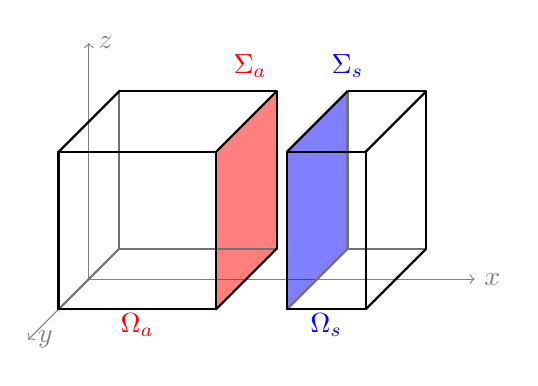
\begin{tikzpicture}[
  scale = 1, 
  cube/.style={thick,black},
  cubebehind/.style={thick,black!55},
  grid/.style={very thin},
  axis/.style={->,gray},
  domain/.style={opacity=.5}
  ]
  
	%draw the axes
	\draw[axis] (0,0,1) -- (3+\ThickStr+\Sep,0,1) node[anchor=west]{$x$};
	\draw[axis] (0,0,1) -- (0,3,1) node[anchor=west]{$z$};
	\draw[axis] (0,0,0) -- (0,0,3) node[anchor=west]{$y$};


	%draw a grid in the yz plane
% 	\foreach \x in {2}%{0,\StepAir,...,2}
% 	\foreach \y in {0,\StepAir,...,2}
% 		\foreach \z in {0,\StepAir,...,2}
% 		{
% 			\draw[grid,red] (\x,\y,0) -- (\x,\y,2);
% 			\draw[grid,red] (\x,0,\z) -- (\x,2,\z);
% 		}
	
	% Draw the domains
	\draw[opacity=.5, fill=red] (2,0,0) -- (2,0,2) -- (2,2,2) -- (2,2,0) -- cycle;
% 	\draw[opacity=.5, fill=green] (2,0,1) -- (2,0,2) -- (2,2,2) -- (2,2,1) -- cycle;
% 	
	\draw[opacity=.5, fill=blue] (2+\Sep,0,0) -- (2+\Sep,2,0) -- (2+\Sep,2,2) -- (2+\Sep,0,2) -- cycle;
% 	\draw[opacity=.5, fill=orange] (2+\Sep,1,0) -- (2+\Sep,2,0) -- (2+\Sep,2,2) -- (2+\Sep,1,2) -- cycle;
	
	%draw the top and bottom of the cube
	\draw[cubebehind] (0,0,0) -- (0,2,0) -- (2,2,0) -- (2,0,0) -- cycle;
	\draw[cubebehind] (0,0,0) -- (0,0,2);
	\draw[cube] (0,0,2) -- (0,2,2) -- (2,2,2) -- (2,0,2) -- cycle;
	
	\node[red] at (1,-.2,2) {$\Omega_a$};
	\node[above left, red] at (2,2.05,0) {$\Sigma_a$};
	
	%draw the edges of the cube
	\draw[cube] (0,2,0) -- (2,2,0);
	\draw[cube] (2,2,0) -- (2,0,0);
	\draw[cube] (0,2,0) -- (0,2,2);
	\draw[cube] (2,0,0) -- (2,0,2);
	\draw[cube] (2,2,0) -- (2,2,2);
	
	%draw a grid in the yz plane
% 	\foreach \x in {2+\Sep}%{2+\Sep,2+\Sep+\demiThickStr,2+\Sep+\ThickStr}
% 		\foreach \y in {0, \StepStr,...,2}
% 			\foreach \z in {0,\StepStr,...,2}
% 		{
% 			\draw[grid,blue] (\x,\y,0) -- (\x,\y,2);
% 			\draw[grid,blue] (\x,0,\z) -- (\x,2,\z);
% 		}
%	\node[above, blue] at (2+\ThickStr+\Sep,2.05,0) {$\Sigma_s^{(2)}$};

	%draw the top and bottom of the cube
	\draw[cubebehind] (2+\Sep,0,0) -- (2+\Sep,2,0) -- (2+\ThickStr+\Sep,2,0) -- (2+\ThickStr+\Sep,0,0) -- cycle;
	\draw[cubebehind] (2+\Sep,0,0) -- (2+\Sep,0,2);
	\draw[cube] (2+\Sep,0,2) -- (2+\Sep,2,2) -- (2+\ThickStr+\Sep,2,2) -- (2+\ThickStr+\Sep,0,2) -- cycle;
	
	%draw the edges of the cube
	\draw[cube] (2+\Sep,2,0) -- (2+\ThickStr+\Sep,2,0);
	\draw[cube] (2+\ThickStr+\Sep,2,0) -- (2+\ThickStr+\Sep,0,0);
	\draw[cube] (2+\Sep,2,0) -- (2+\Sep,2,2);
	\draw[cube] (2+\ThickStr+\Sep,0,0) -- (2+\ThickStr+\Sep,0,2);
	\draw[cube] (2+\ThickStr+\Sep,2,0) -- (2+\ThickStr+\Sep,2,2);
% 	
	\node[blue] at (2.5+\Sep,-.2,2) {$\Omega_s$};
	\node[above, blue] at (2+\Sep,2.05,0) {$\Sigma_s$};
	
\end{tikzpicture}
